% ----------------------------------------------------------------------

\newpage

\subsection{\gainped Test}
\label{ss:gainped}

\subsubsection{Purpose}

The \gainped test does not alter any \dac parameters,
but merely evaluates the shape of the pulse height vs. \vcal distribution for each pixel.
For each pixel, the distribution is fitted and the fit parameters are stored for later use.
Since variations in gain are expected between pixels in a \roc,
the gain must be measured independently for each pixel so that the pulse height to be calibrated back to the input signal size, 
in units of the \vcal~\dac (high range).

\subsubsection{Methodology}

For each pixel, the pulse height is sampled for a variety of \vcal values.
In the low \vcal range, the PH is measured in steps of 10 DAC units (configurable), from 10 to 255.
Then, in the high \vcal range, the PH is measured for values of 30,50,70,90, and 200.
The results of these two scans are then combined into a PH vs. \vcal curve over the full \vcal range.
This curve converts the high range \vcal values to their larger low range equivalents by multiplying by a factor of seven.
This curve is then fit using an error function, and the four fitted parameters, along with their errors, are recorded.
Parameter 0 corresponds to the \vcal value at the center of the error function, when the PH is halfway between zero and saturation (255).
Parameter 1 is proportional to the width of the turn-on, and, as such, is inversely related to the gain of the pixel.
Parameter 2 shifts the error function upwards, with a value of unity moving the floor of the function to zero.
Parameter 3 corresponds to half the height of the function, and should be near 127.5 (255/2).
The \roc-wide distributions for these four parameters 
and their relative errors are shown in Figures~\ref{fig:gainped_gainPedestalP0}-\ref{fig:gainped_P3_relErr}.
Additionally, these parameters are stored for later use in text files with names of the form ``phCalibrationFitErr35\_C\#.dat''
(assuming the module was trimmed to \vcal=35).
Finally, the linearity of the pixel's response is estimated.
Using the fitted error function, the true integral of the function in the \vcal range from 0-200 (low range) is compared to a linear approximation.
The quotient of these two values should be near unity for a linearly-responding pixel.
The \roc-wide distribution of this quantity, dubbed the ``non-linearity'', is shown in Figure~\ref{fig:gainped_gainPedestalNonLinearity}.

\subsubsection{Output}

\begin{figure}[!htp]
\centering
\begin{minipage}{0.45\textwidth}
  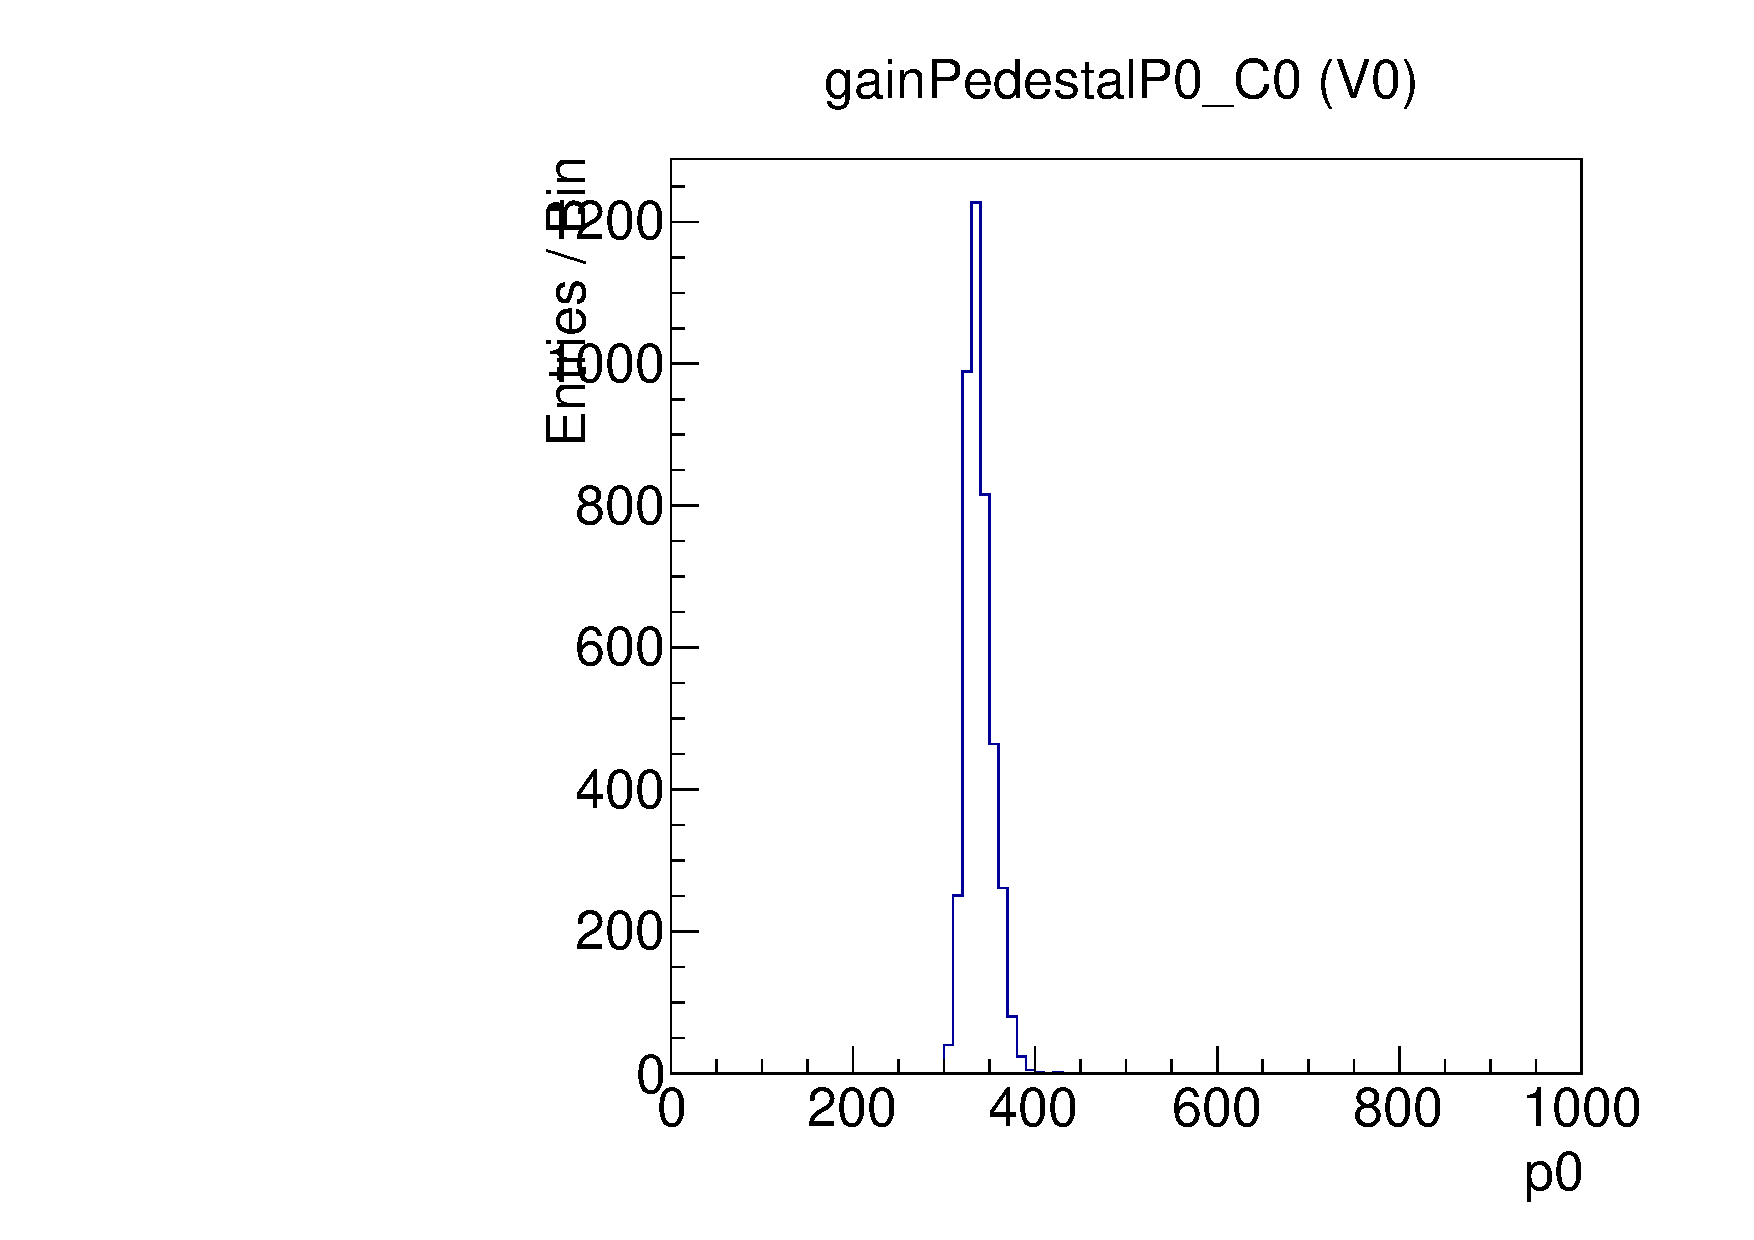
\includegraphics[width=1.0\textwidth]{figures/gainped_gainPedestalP0.pdf}
  \caption{Distribution of fitted values of parameter 0, the \vcal center of the fitted error curve.}
  \label{fig:gainped_gainPedestalP0}
\end{minipage}
\hspace{0.3cm}
\begin{minipage}{0.45\textwidth}
  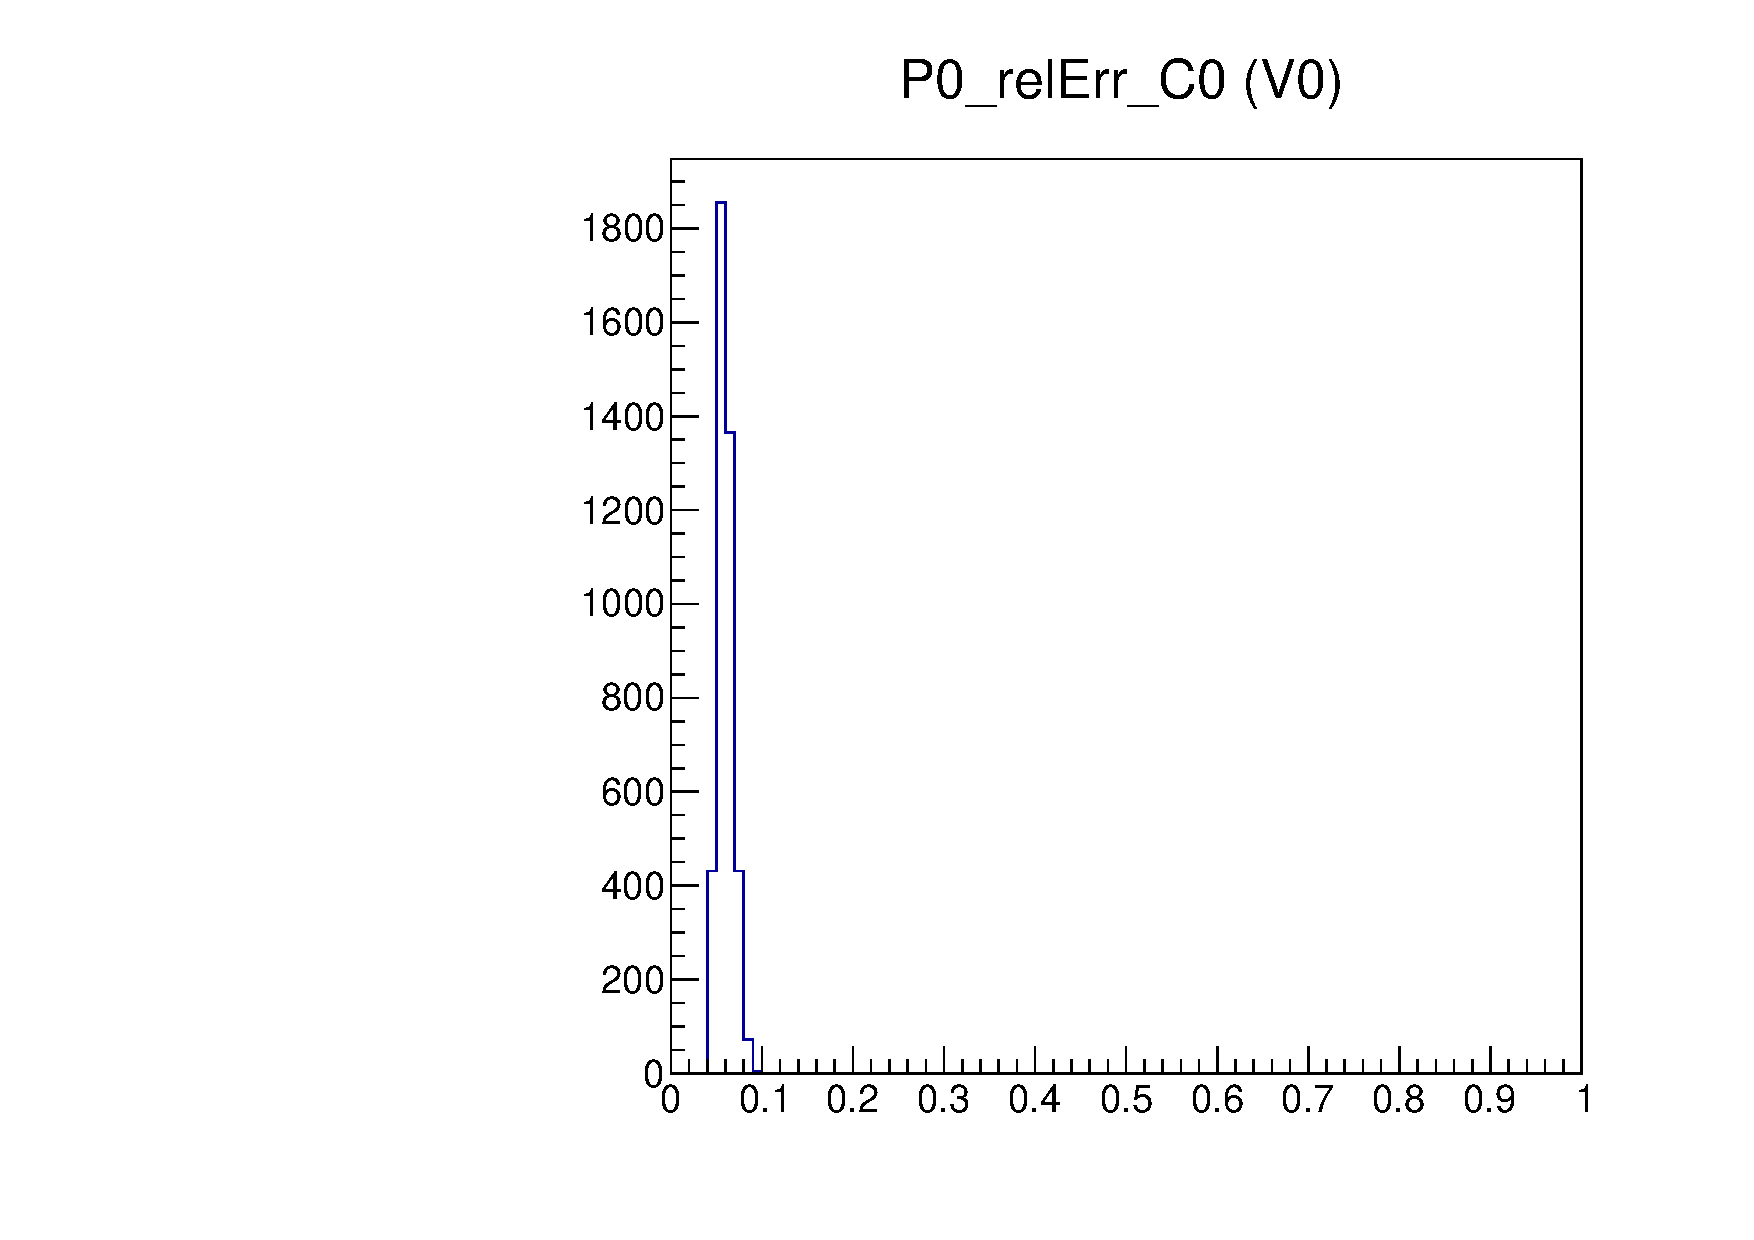
\includegraphics[width=1.0\textwidth]{figures/gainped_P0_relErr.pdf}
  \caption{Relative errors on the fitted values of parameter 0.}
  \label{fig:gainped_P0_relErr}
\end{minipage}
\end{figure}

\begin{figure}[!htp]
\centering
\begin{minipage}{0.45\textwidth}
  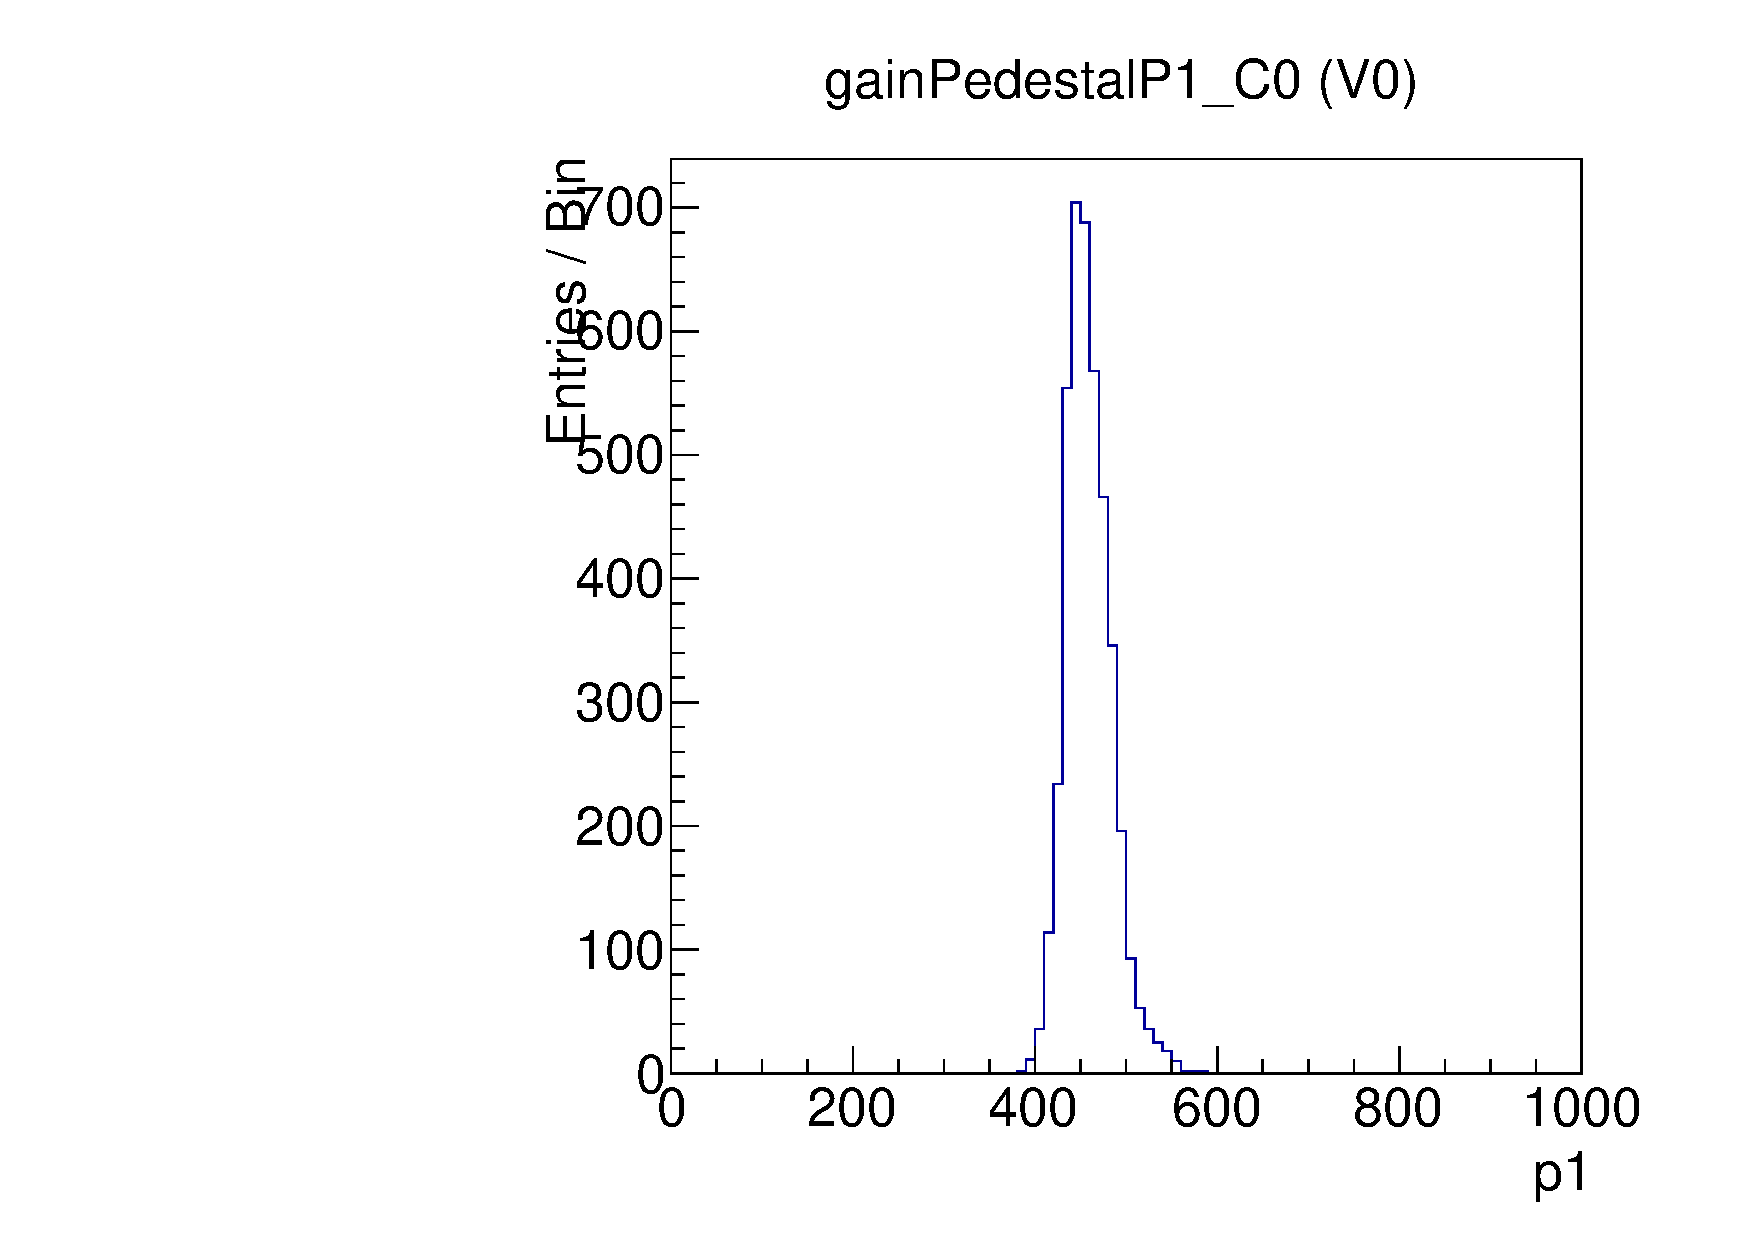
\includegraphics[width=1.0\textwidth]{figures/gainped_gainPedestalP1.pdf}
  \caption{Distribution of fitted values of parameter 0, related to the error function width.}
  \label{fig:gainped_gainPedestalP1}
\end{minipage}
\hspace{0.3cm}
\begin{minipage}{0.45\textwidth}
  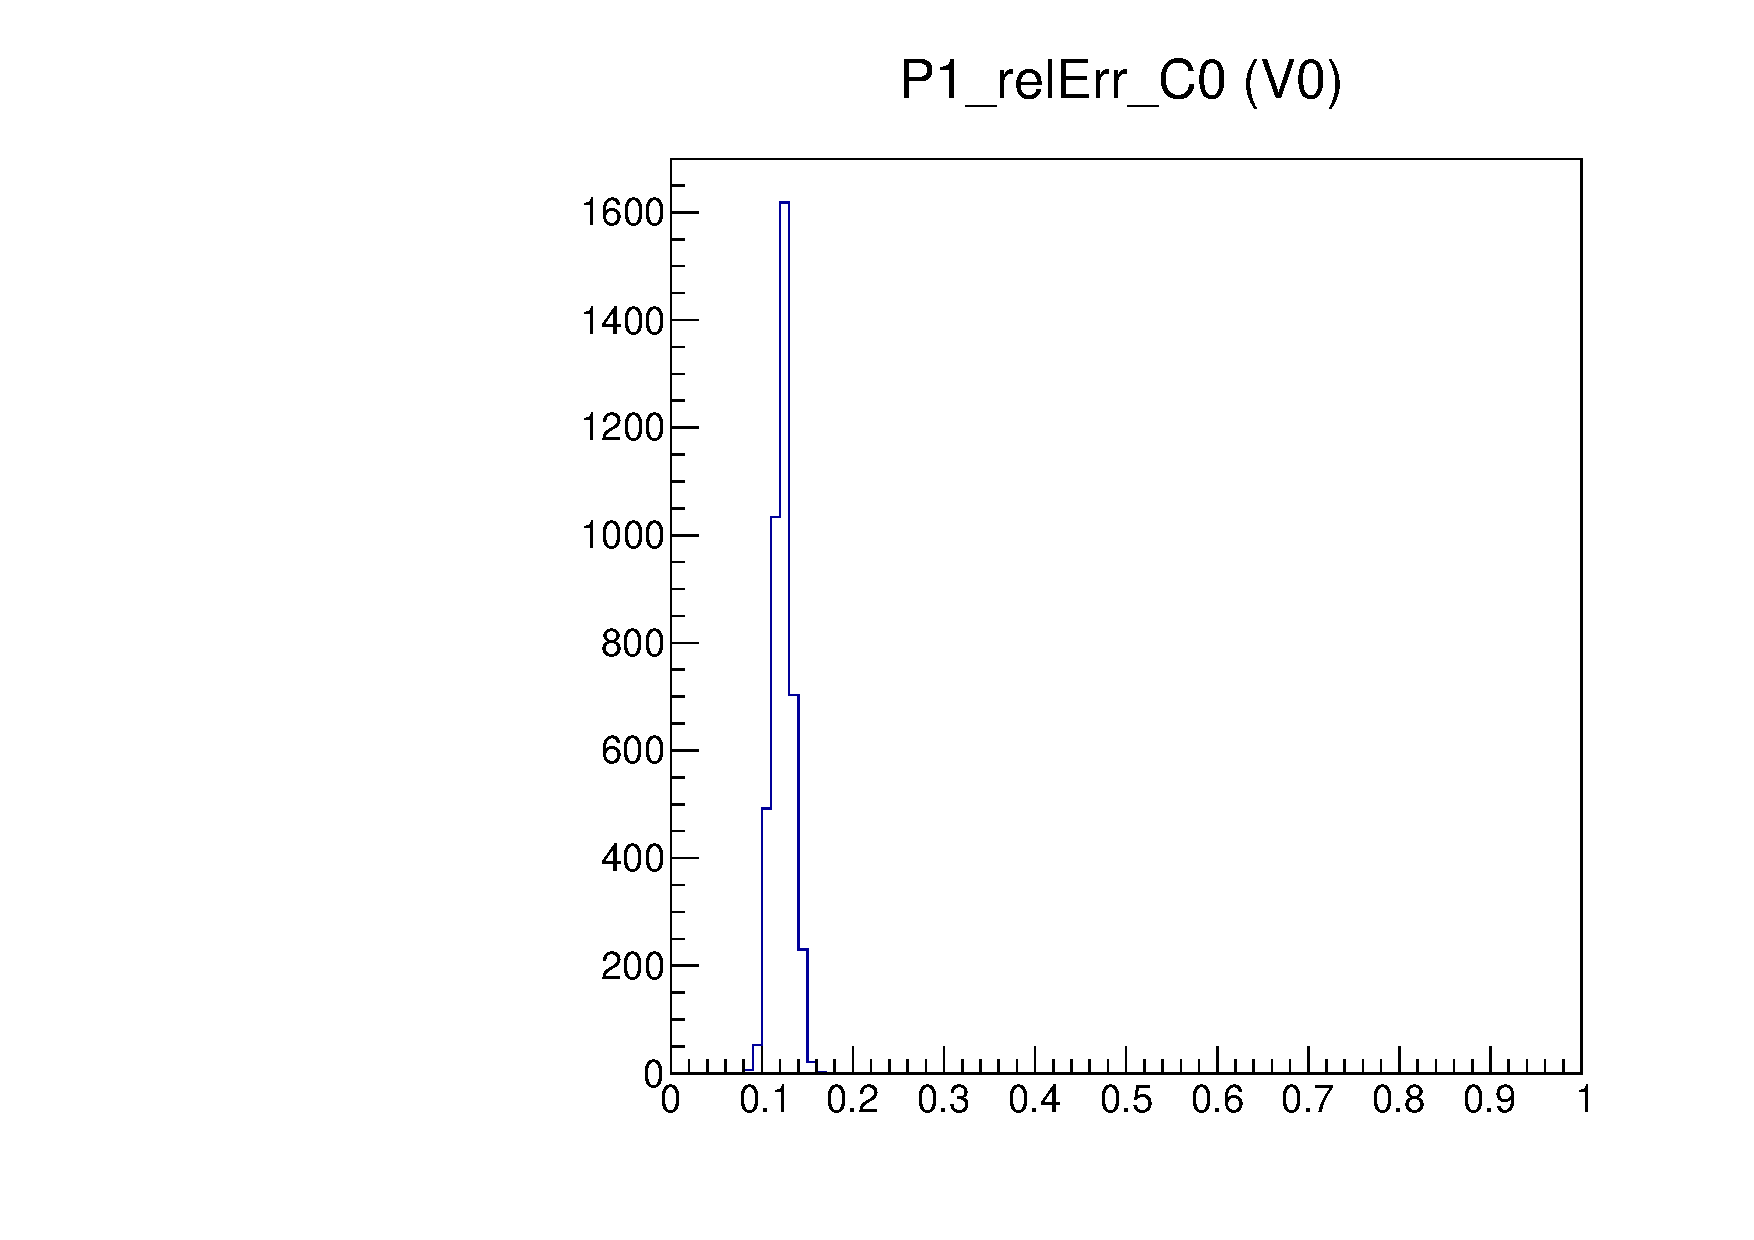
\includegraphics[width=1.0\textwidth]{figures/gainped_P1_relErr.pdf}
  \caption{Relative errors on the fitted values of parameter 1.}
  \label{fig:gainped_P1_relErr}
\end{minipage}
\end{figure}

\begin{figure}[!htp]
\centering
\begin{minipage}{0.45\textwidth}
  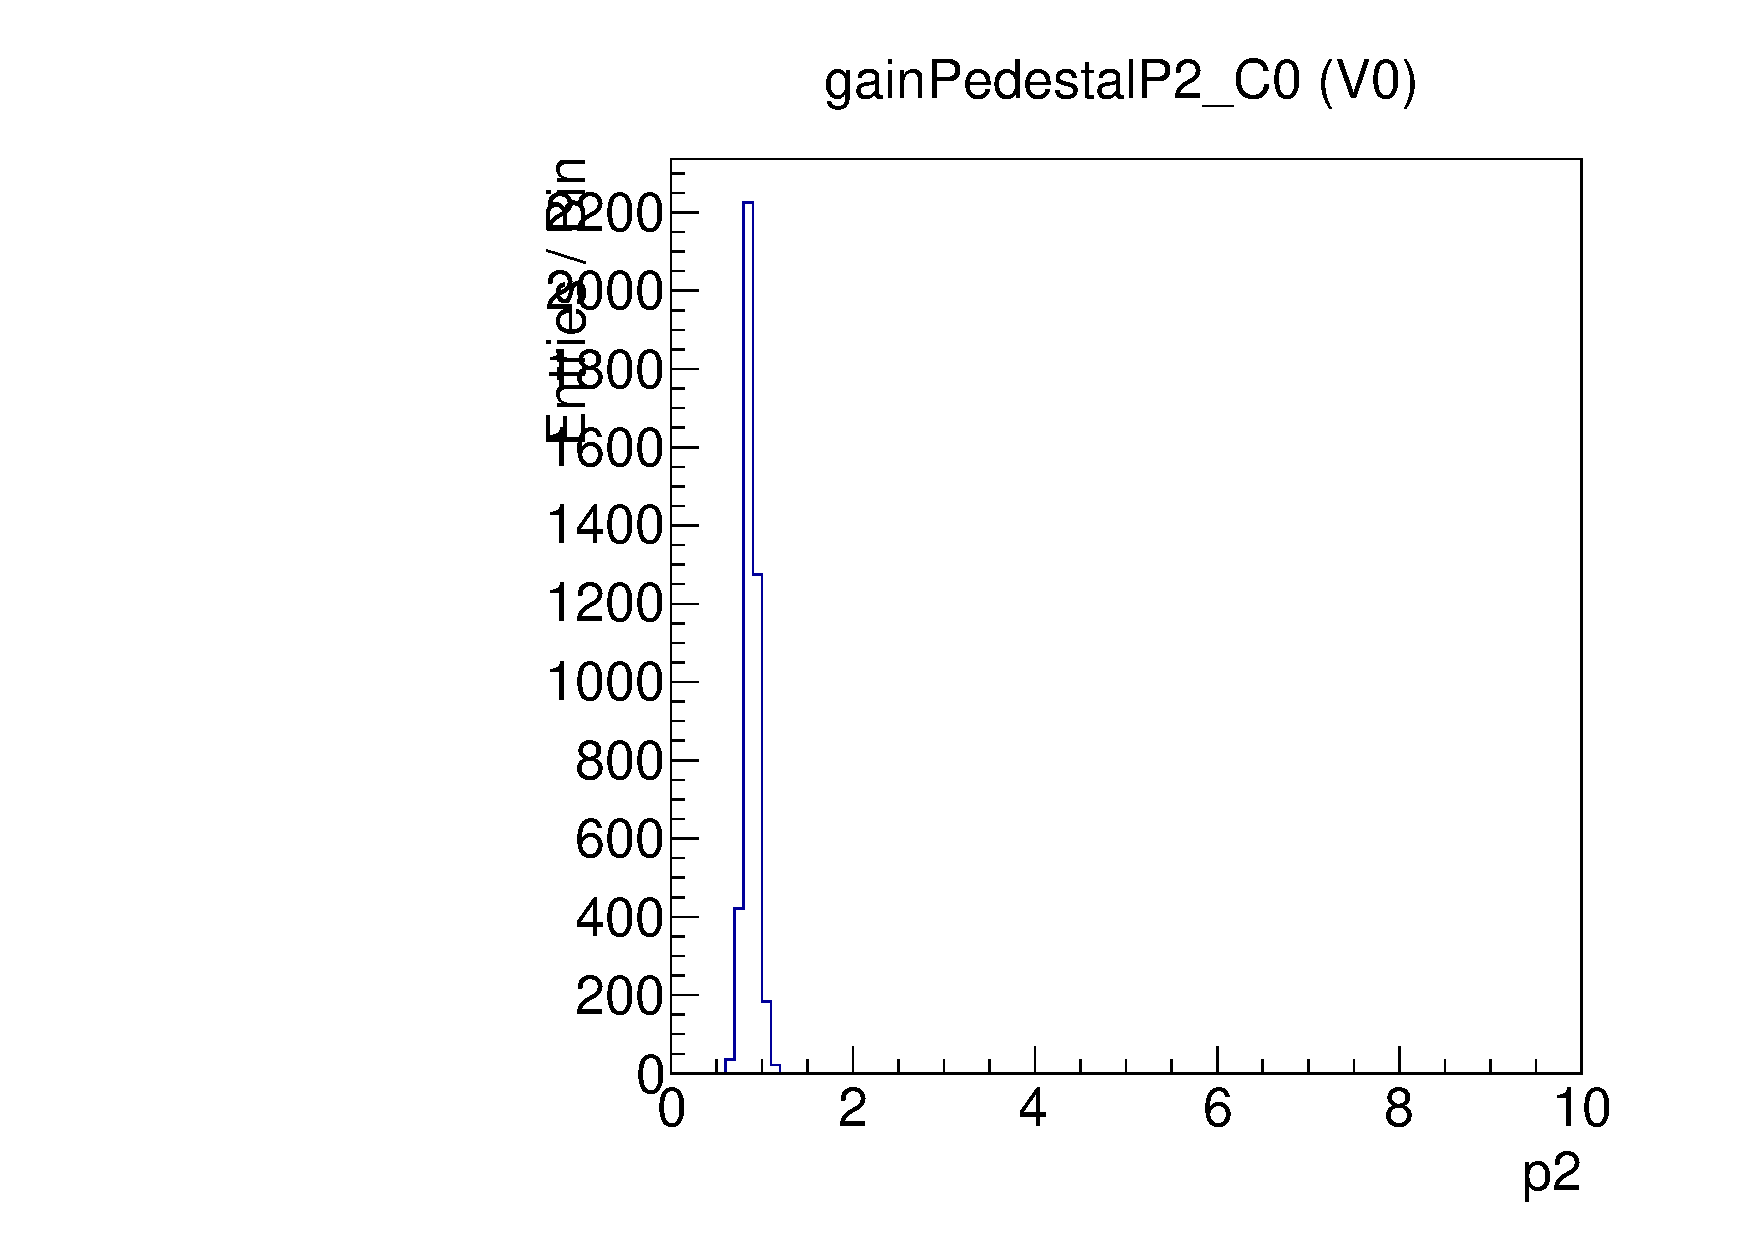
\includegraphics[width=1.0\textwidth]{figures/gainped_gainPedestalP2.pdf}
  \caption{Distribution of fitted values of parameter 2, the vertical shift in the error function.}
  \label{fig:gainped_gainPedestalP2}
\end{minipage}
\hspace{0.3cm}
\begin{minipage}{0.45\textwidth}
  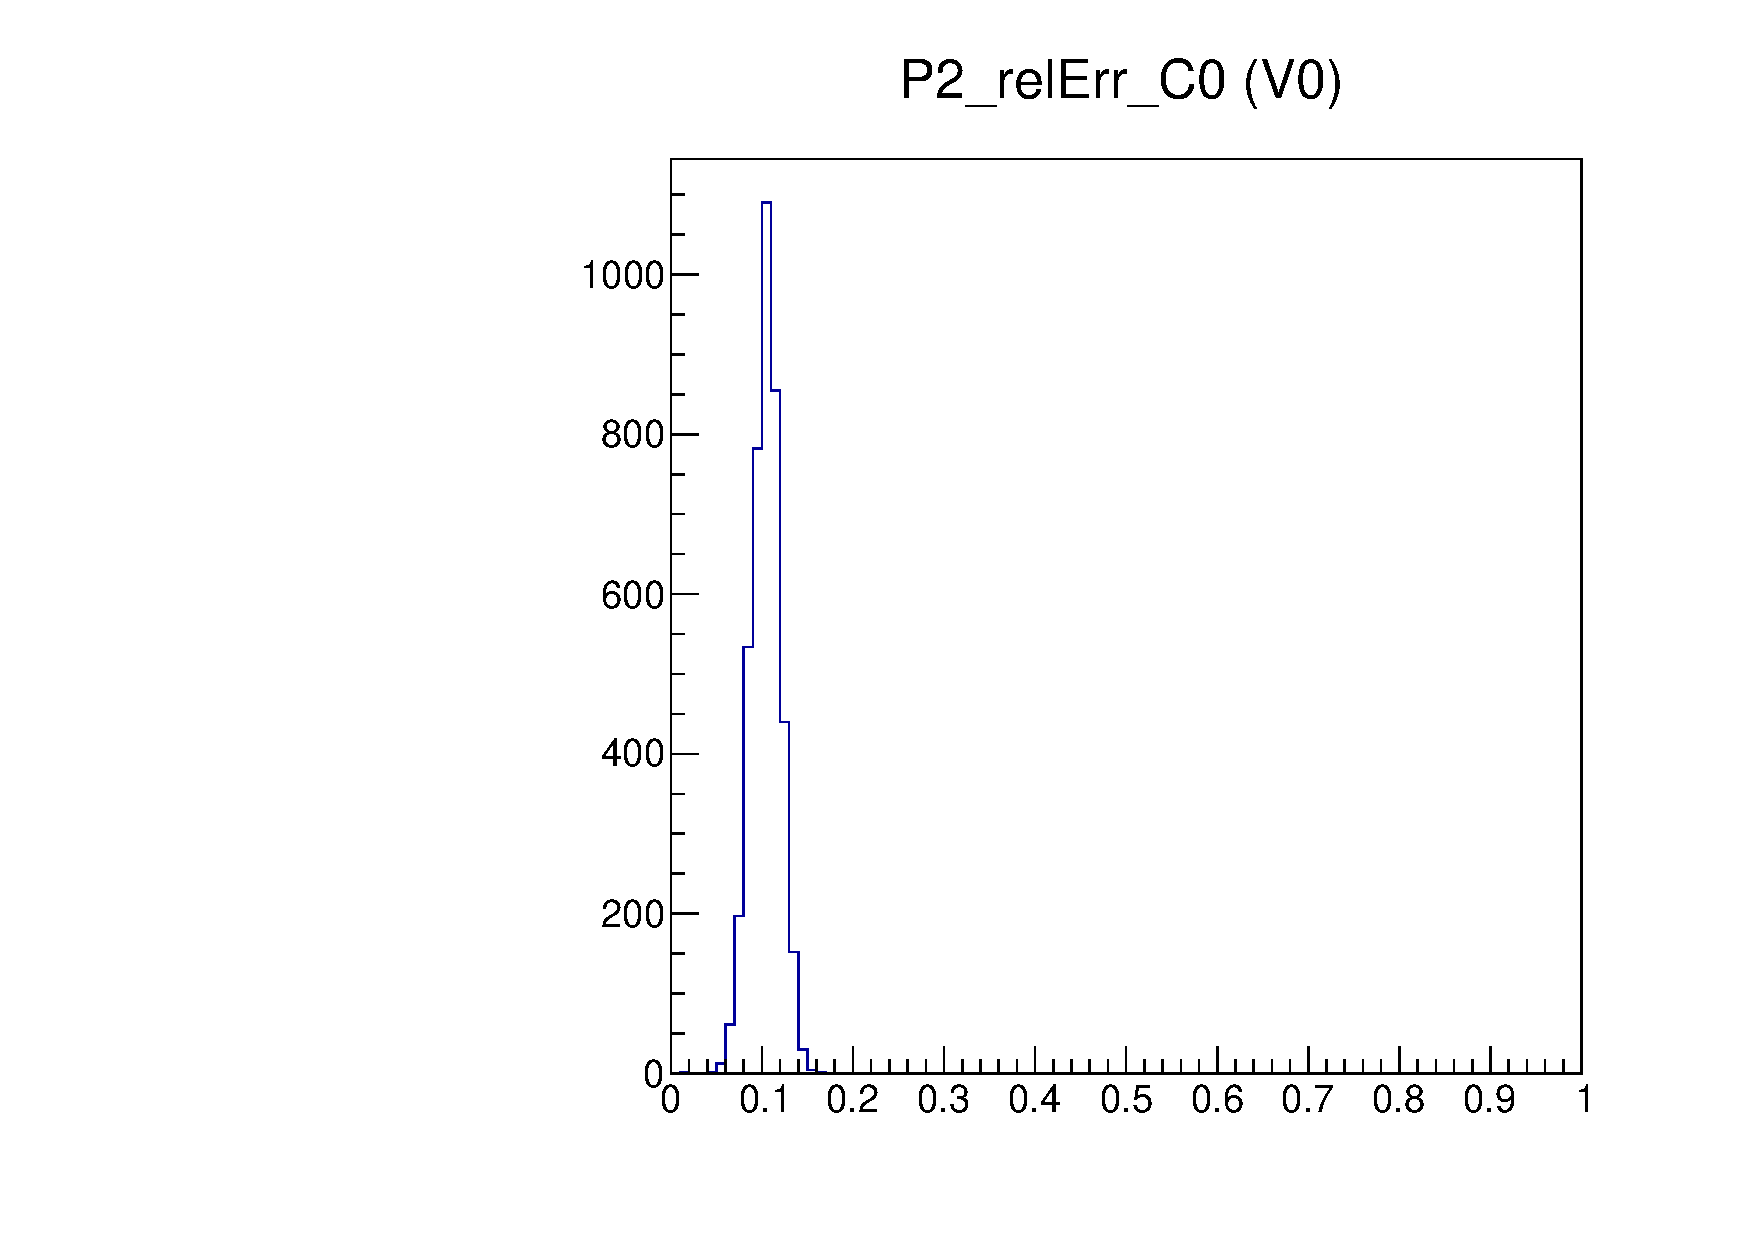
\includegraphics[width=1.0\textwidth]{figures/gainped_P2_relErr.pdf}
  \caption{Relative errors on the fitted values of parameter 2.}
  \label{fig:gainped_P2_relErr}
\end{minipage}
\end{figure}

\begin{figure}[!htp]
\centering
\begin{minipage}{0.45\textwidth}
  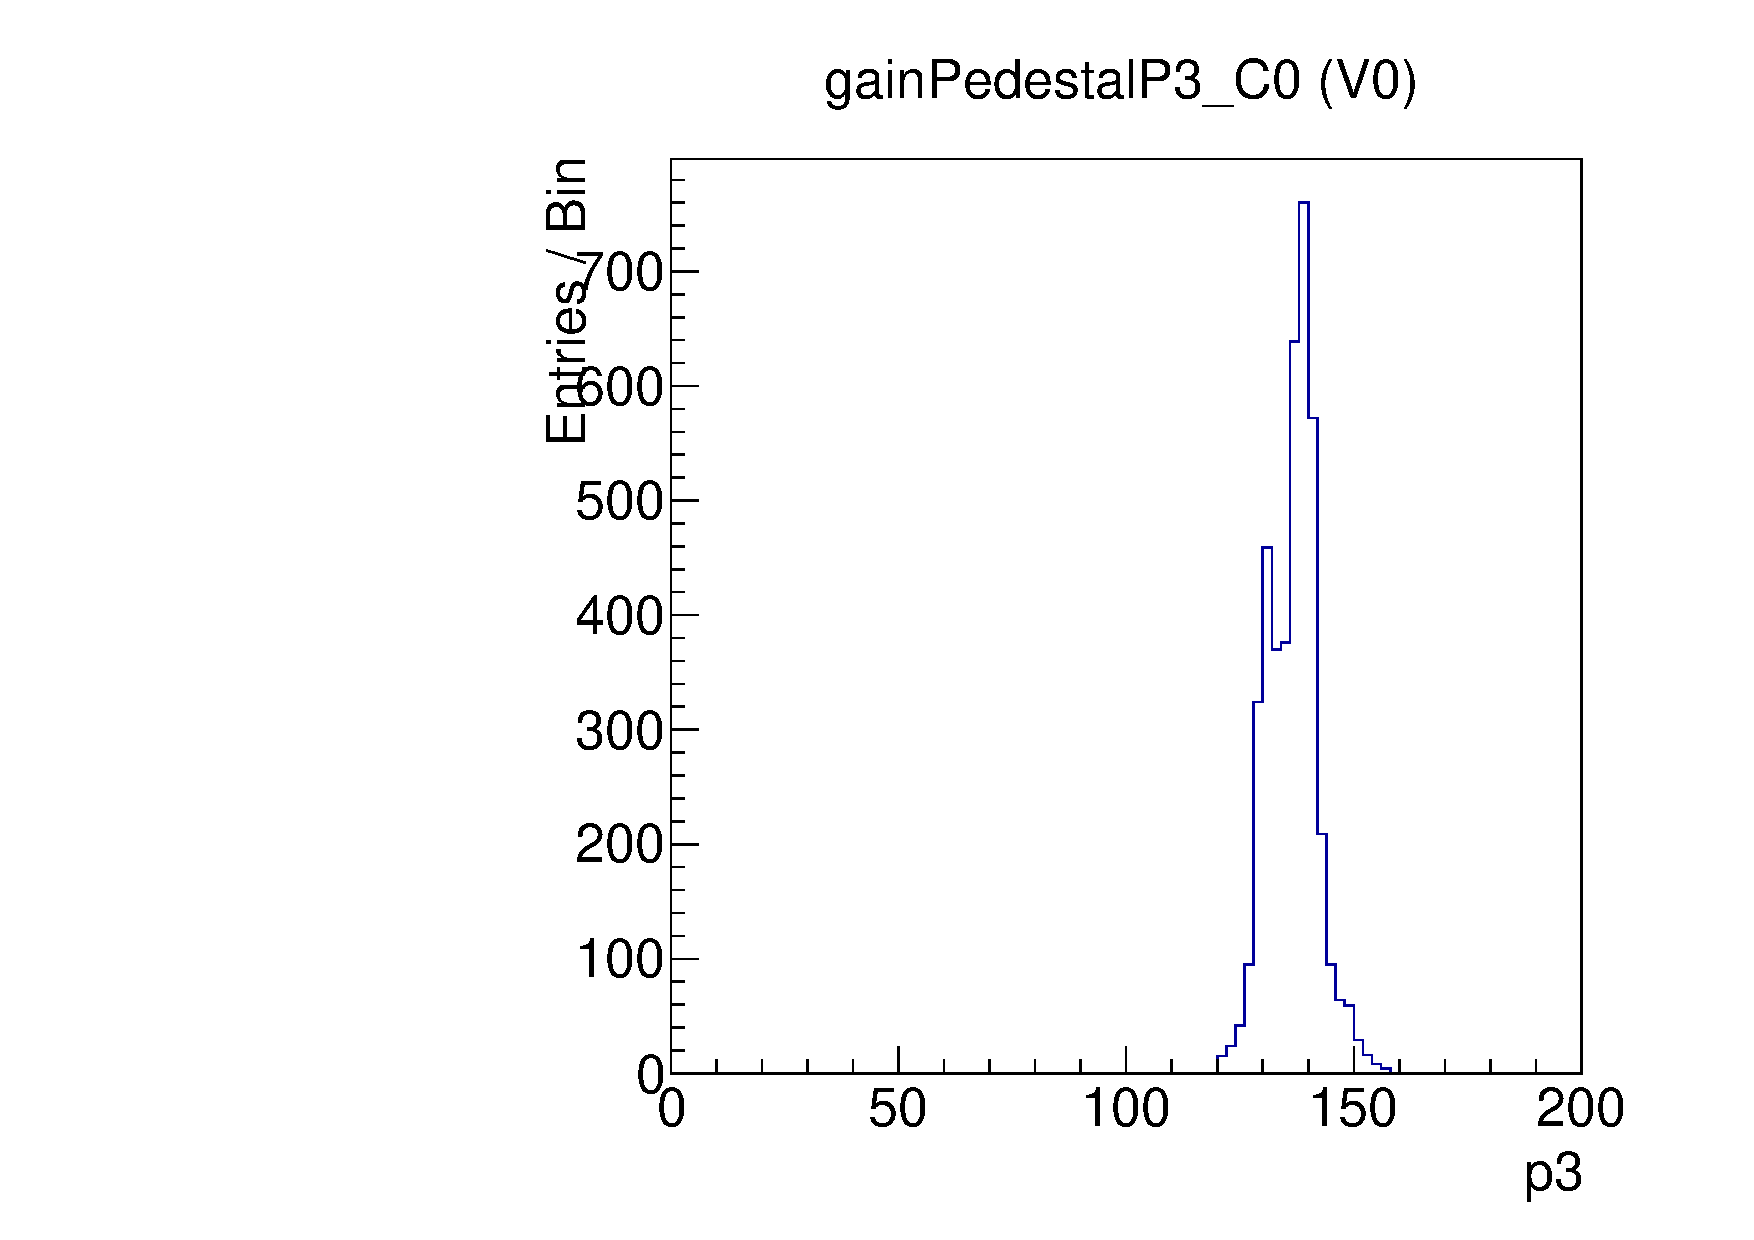
\includegraphics[width=1.0\textwidth]{figures/gainped_gainPedestalP3.pdf}
  \caption{Distribution of fitted values of parameter 3, equal to half the height of the error function plateau.}
  \label{fig:gainped_gainPedestalP3}
\end{minipage}
\hspace{0.3cm}
\begin{minipage}{0.45\textwidth}
  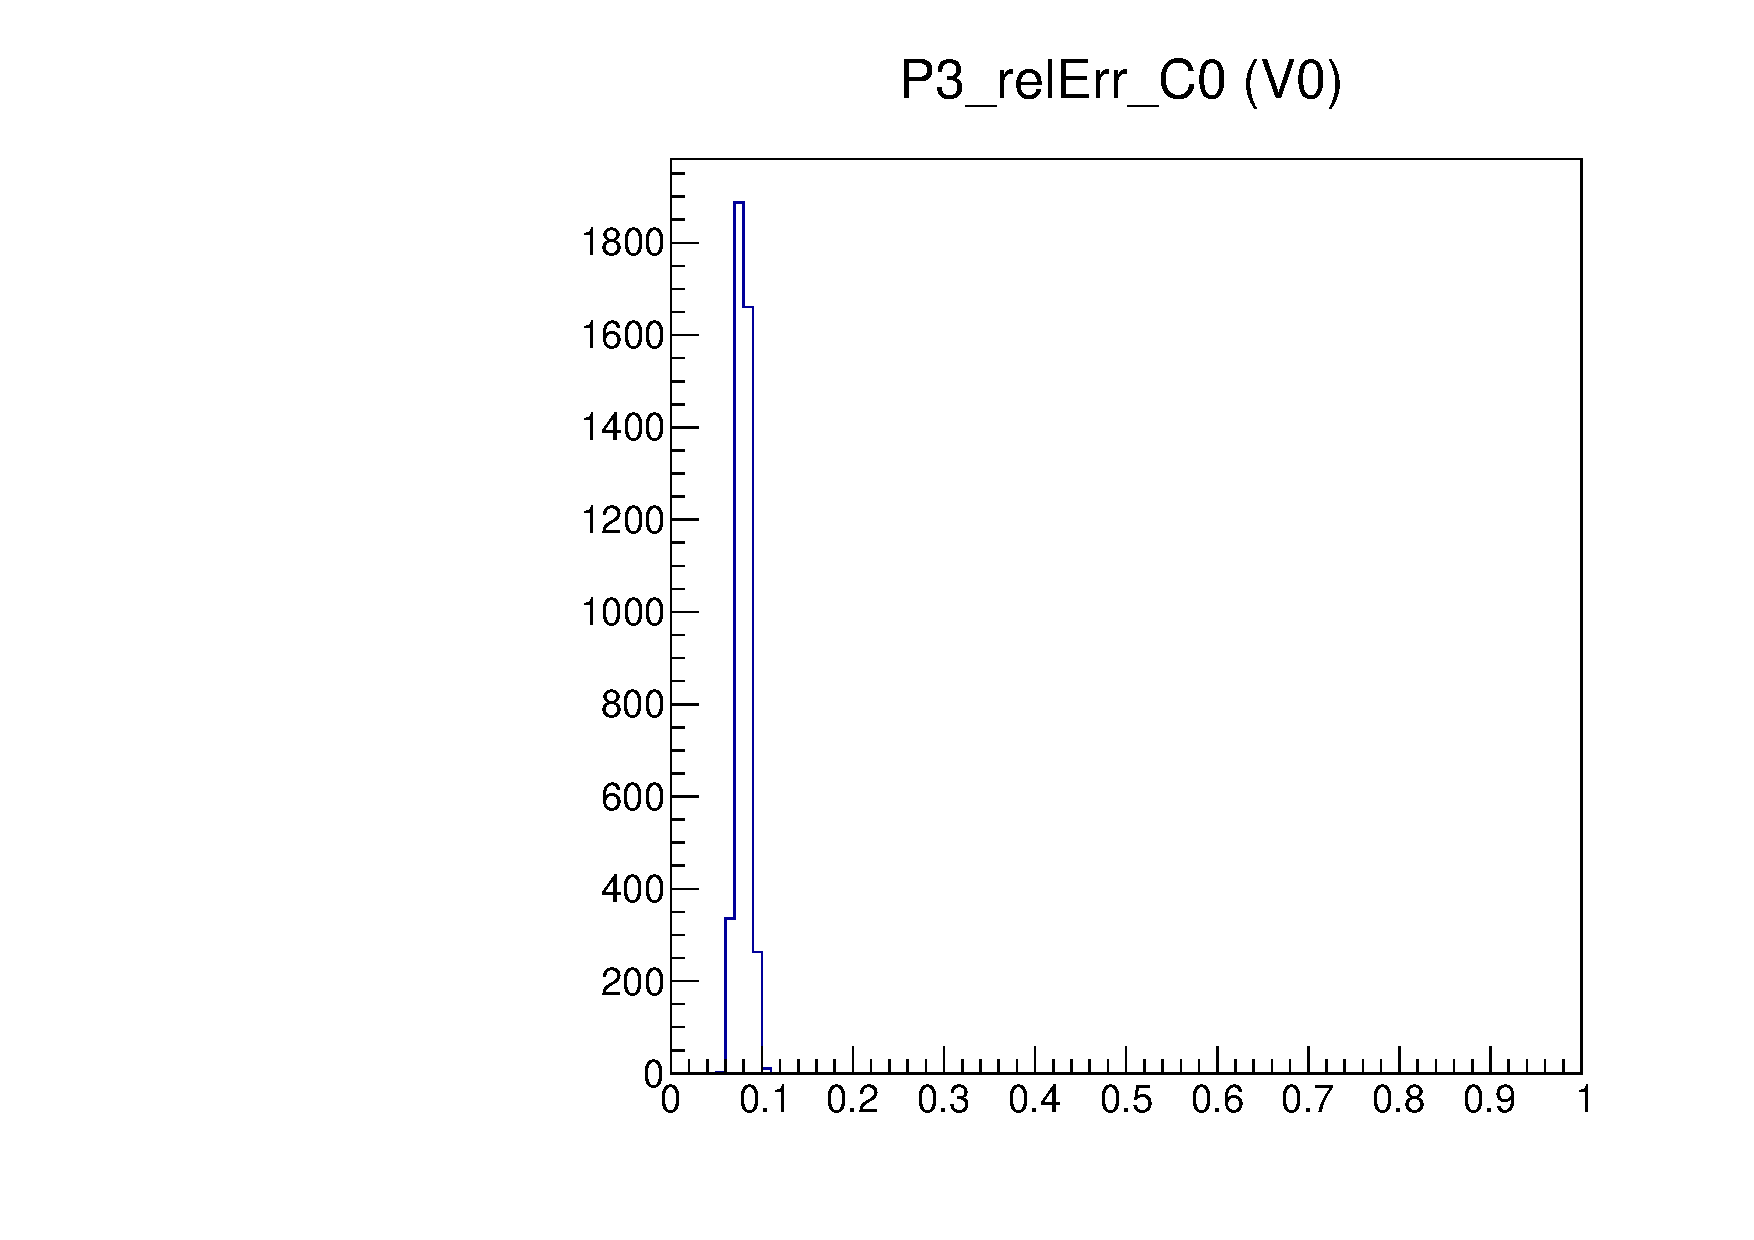
\includegraphics[width=1.0\textwidth]{figures/gainped_P3_relErr.pdf}
  \caption{Relative errors on the fitted values of parameter 3.}
  \label{fig:gainped_P3_relErr}
\end{minipage}
\end{figure}

\begin{figure}[!htp]
\centering
\begin{minipage}{0.45\textwidth}
  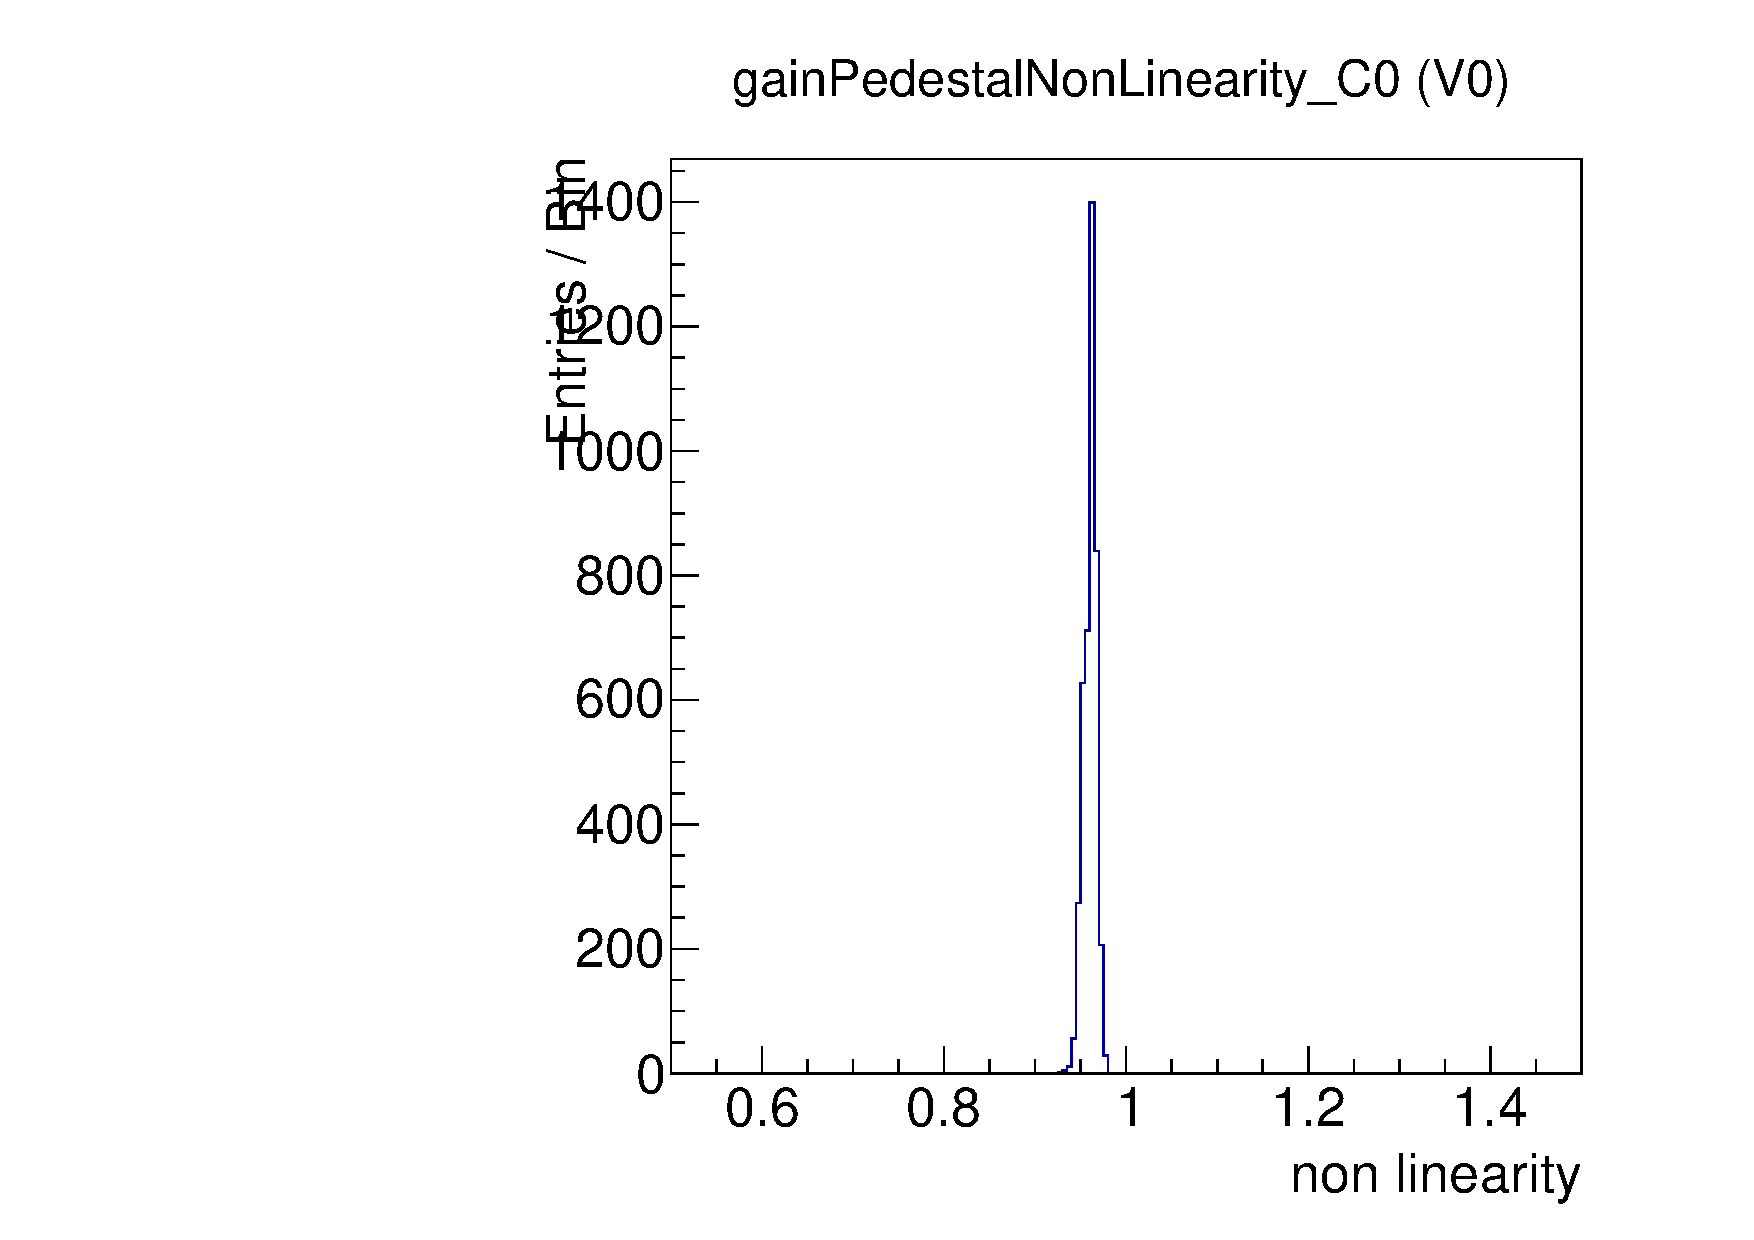
\includegraphics[width=1.0\textwidth]{figures/gainped_gainPedestalNonLinearity.pdf}
  \caption{Non-linearity is defined as the ratio of the integral of the fitted error function to the integral of a linear approximation,
           in the \vcal range from 0-200 (low range).}
  \label{fig:gainped_gainPedestalNonLinearity}
\end{minipage}
\end{figure}
